\documentclass[11pt,a4paper]{article}
\usepackage{named}
\usepackage[pdftex]{graphicx}
\usepackage{graphics}
\usepackage{subfig}
\usepackage{newlfont}
\usepackage{amssymb}
\usepackage{amsmath,amsthm}
\usepackage{alltt}
\usepackage{hyperref}
\hypersetup{colorlinks=true,				% set this to false when printing
linkcolor = black,	 			%Color for normal internal links.
anchorcolor = black, 		%Color for anchor text. 
citecolor = blue, 			%Color for bibligraphical citations in text. 
filecolor = magenta, 			%Color for URLs which open local �les. 
menucolor = blue,			%Color for Acrobat menu items. 
urlcolor = blue, 				%Color for linked URLs. 
}


\pagestyle{headings}

%\documentstyle[subsections]

\def\nonumchapter#1{%
    \chapter*{#1}
    \addcontentsline{toc}{chapter}{#1}}

\def\baselinestretch{1.3}\large\normalsize
\setlength{\textwidth}{14cm}
\setcounter{secnumdepth}{4}
\setcounter{tocdepth}{4}

\newcommand{\Robocup}{\textnormal{RoboCup}\unskip}
\newcommand{\RoboCup}{\textnormal{RoboCup}\unskip}
\newcommand{\NUbot}{\textnormal{NUbot}\unskip}
\newcommand{\Nubot}{\textnormal{NUbot}\unskip}
\newcommand{\NUbots}{\textnormal{NUbots}\unskip}
\newcommand{\Nubots}{\textnormal{NUbots}\unskip}
\newcommand{\aibo}{\textnormal{AIBO}\unskip}
\newcommand{\AIBO}{\textnormal{AIBO}\unskip}
\newcommand{\fourlegged}{\textnormal{Four-Legged League}\unskip}


\title{The 2009 Nubots Team Report}
\author{ Naomi Henderson \and Steven P. Nicklin \and Aaron Wong \and Jason Kulk \and Stephan K. Chalup \and Robert King}

\begin{document}

\maketitle

\begin{figure}[!h]
\begin{center}
   \leavevmode
    \scalebox{0.2} {
\includegraphics{figs/NUMANOIDS.jpg} }
    \label{fig:NUMANOIDS}
\end{center}
\end{figure}


\begin{center}
School of Electrical Engineering \& Computer Science\\
The University of Newcastle, Callaghan 2308, Australia \\
\url{http://www.robots.newcastle.edu.au}\\

\end{center}
\newpage

\tableofcontents
\newpage

\section{Introduction}

\subsection{Overview}

The NUbots from the University of Newcastle, Australia have had a strong record of success in the RoboCup Four Legged League since first entering in 2002. The Nubots achieved 3rd place in 2002 (Fukuoka), and again in 2003 (Padua) and 2004 (Lisbon). In 2005 (Osaka) with a complete redevelopment of the code, the NUbots came 2nd in a heartbreaking penalty shoot out against the German Team. With a strong 2005 base code, 2006 development focused on debugging and fine tuning. The result was a nail biting final against rUNSWift in Bremen where the NUbots won 7-3. Code development plateaued in 2007 and we lost the final in Atlanta against the Northern Bites.  

2008 Involved the transition from the Sony ERS-7 robot to the Aldebaran Nao. We also created a joint team, The NUManoids with the the National University of Ireland, Maynooth (NUIM). Together we successfully overcame the challenges of adapting to the new hardware to become the first world champions of the Robocup Nao SPL.

For 2009 we separated from NUIM two create two independent teams and once again became the NUbots. We set out to improve the previous years code. The league as a whole made a great leap forward compared to the previous year. With major improvements to our vision, localisation and locomotion it was not enough to defend our title. We completed the competition with a ranking of quarter finalist.

This report will outline the system and some more recent advances added into the system for the 2009 RoboCup competition.

\subsection{Software Layout}

Our 2009 system was based on last years architecture \cite{NUManoids2008} which originated from the Sony Aibo architecture in 2006 \cite{NUBOT2006}. Our system consists of one control module \emph{Nao} and four functional modules -
\emph{Vision, Localisation, Behaviour and Locomotion}. 

The flow of information in our system can be seen in Figure
\ref{fig:software}. 

\begin{figure}[!ht]
\begin{center}
    %\leavevmode
    \scalebox{0.5} {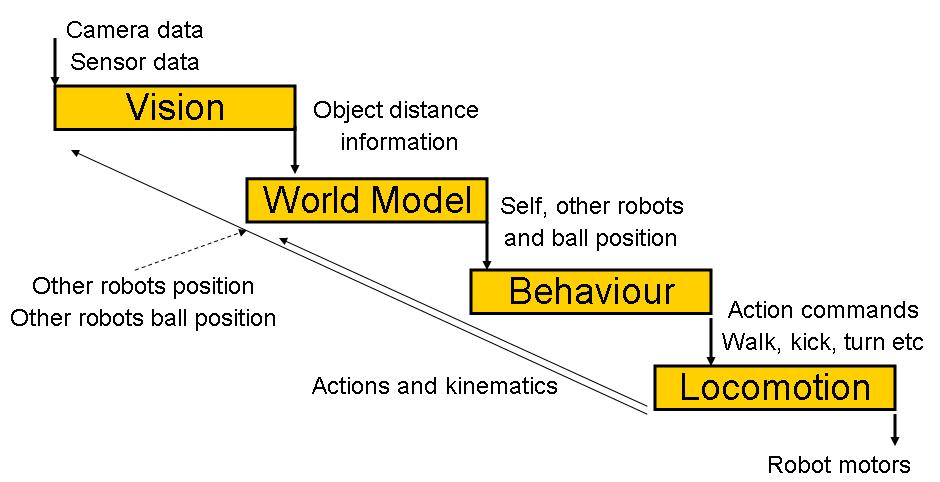
\includegraphics{figs/software.jpg} }
    \caption{2009 Software Architecture}
    \label{fig:software}
\end{center}
\end{figure}


\section{Vision}
The Nao vision system followed the process: \emph{Input image, classify image, form blobs, sort colour blobs, combine soft blobs, find ball, find goals, detect lines}. The 2009 vision module was an advancement over the 2008 module. This section details the main functions of the vision system and the reasons behind them. 

\subsection{Overview}

Webots was used to develop the base vision system in 2008. Inputting the RGB image and classifying it using a perfect look-up table (LUT) allowed blob formation and basic object recognition to be tested which then allowed for localisation development to begin. 

However this was not required in 2009, as the vision debugging application \emph{Eye of the NUbot} (EOTN) was already compatible with the robot directly. An advancement of EOTN carried over from last year was the HSI classification method. Transforming the YUV image to HSI values and selecting the classification region in HSI allowed for an intuitive classification method and better separation of hue ranges. 

%The process of setting up a robot for a game includes setting the camera settings were selected using \emph{Telepathe}. 
Calibration of the vision system included selecting camera settings for the field using \emph{Telepathe}.
Then obtaining image streams which were saved on the robot or could be transferred through the wireless interface to EOTN to be processed and examined. During examination of the images, the user could also generate a LUT using EOTN. Generating the LUT also enabled the user to check the classification and field object detection for errors. A generated LUT could then be uploaded to the robot for use. This had to be completed for both top and bottom cameras.

Advancements that were included in the vision module this year were increased ratio checks for the ball and goals, including a green horizon. This was to reduce the number of false objects recognised by the robots in between the horizon line and the field. We also included heuristics for the detection of new field objects, such as penalty spots and the centre circle. These new field objects greatly enhanced the performance of the localisation module. Also, we increased the camera resolution from the minimal of 160x120 to a medium image resolution of 320x240. This increased the accuracy of the object seen (example, a ball can be seen at the full length of the field), with a trade-off to robots processing speed. Also there was an additional camera added into the hardware system, in which we had to account for when processing the image.

%\emph{Input image, classify image, form blobs, sort colour blobs, combine soft blobs, find ball, find goals, line detection}


\subsection{Image Quality and Camera Settings}
%One good thing about the transition from the Aibo to the Nao was the improvement in camera quality. While the camera still had its share of problems, such as random swaps of U and V channels, random blackouts and random ghost camera settings, at least it made the separation of colours easier.
%The Nao has three different resolutions for which we could obtain images, 160x120, 320x240 and its native resolution 640x480. 
This year was the first year where we successfully started processing larger image resolutions. We increased the image resolution from 160x120 pixels to double the resolution, 320x240 pixels. This enabled clearer images and more accurate distances when we found recognisable objects. For example a ball could be detected by the goal keeper standing at its goal from the other end of the field. However, with higher resolution images the calculations to process an image became computationally heavy. This forced us to reduce our frame rate to 15 frames per second.

There was an additional camera installed around the nose of the Nao. This camera was particularly useful for lining up kicks. However, switching over from one to another would take time, which equates to the loose of a few frames. Logic was inserted in the search behaviour to reduce the number of camera transitions. 

\subsubsection{Camera settings}

The Nao camera has 6 main camera settings with a large range of values for each setting. This means that the camera settings are very sensitive to lighting changes and not only do colour tables need to be recalibrated for any change, but also the camera settings. At the RoboCup venue the camera settings and colour tables had to be recalibrated for both the main field and test fields. 

The robot is mobile with a movable head. This means that images are subject to blurring and lighting flare. Camera settings are chosen to minimise blurring and allow for best colour separation.

\subsection{Colour Classification}

Colour classification is the top tier in the software system. Any error in classification has a flow on effect to the entire system. Image pixels are mapped to a colour class by referencing a LUT. The environment of the Standard Platform League is colour coded so that objects are recognisable by colour. Rather than classify pixels based on object colour classes alone, additional `soft' colour classes are used to allow additional colour information to be classified and to reduce the risk of false positive classification.

\subsubsection{Soft Colour Classification}

Soft colour classification is used to classify regions of colour that belong to an object but is less saturated due to lighting conditions or overlaps with another colour class. This allows the decision about what object the soft colour belongs to, to be delayed until the entire image is processed.

Using soft colour allows for the classification of `noisy' shades of colour and allows valuable object size information to be kept. The risk of false positives is reduced by allowing true colour to be classed as the shades of colour that are highly saturated. Object decisions are based on the presence of true colour and then soft colour can be used for additional size information.

The shiny bright blue uniforms of the Nao have created a significant overlap of colour values with the blue goal. Similarly, the shiny red uniforms become less saturated with the reflection of light and the hue values shift closer to orange.

Soft colour is also applied to less saturated shades of colour. These shades are more likely to occur in background noise. Soft colour is used to classify additional bright and dark shades of red, orange, yellow and blue. 
 
Blobs are formed for each colour class, including soft colours. Once the image is processed soft colour decisions are made based on blob arrangement in Soft Colour Filtering. 

\subsection{Blob Formation}

Grouping of classified colours is used for the transfer of information from an image to object recognition. When forming blobs the colour, size and area information is required. Blobs are formed based on classified colour of the classified image. Undefined, white and field green and the soft colour shadow-black are not included in blob formation. This is due to the fact that size and shape information is not required for objects of these colours. It is also due to the nature of distribution of these colours. They are all abundantly spread throughout images and scattered; forming blobs on images would involve unnecessary processing. 

Blob formation checks every pixel of the image when forming blobs, this means we can form blobs as small as 1x1, however, we only use blobs greater than or equal to 3x3 pixels. 

\subsection{Sort Colour Blobs}

Soft colour blobs are filtered and kept if of sufficient size or overlapping with the corresponding true colour. During this stage, a simple check is also performed on the ball object. The ball must sit below the highest green transition (a simple green horizon) to be a valid ball.

\subsection{Combine Soft Blobs}

Overlapping soft colour blobs are merged. Colour blob clusters are then made to prepare information for object recognition. Cluster variables include: exists, correct pixels, colour 2 correct pixels, min x, max x, min y, max y, height, width, area. 
Yellow blobs, shadow yellow blobs and all yellow blobs are clustered for yellow goal recognition. Blue blobs, shadow blue blobs and all blue blobs are clustered for blue goal recognition and blue robot separation. Red blobs and shadow red blobs are clustered for red robot detection.

Clustering allows object recognition to have a region of interest. With the use of soft colour most goal images are made of multiple blobs.
\subsection{Ball Recognition}

Ball recognition was based on previous code. The main difference is that we don't have to deal with the up close ball situation. Instead we have to be able to see the ball at an elevated position and with additional glare shining off the ball. A confidence system is used to decide the ball. Confidence is weighted based on correct pixel to size ratio, size and circle fit.

\subsubsection{Ball Distance, Bearing and Elevation Calculations}
The raw values of bearing and elevation are calculated using the centre x and centre y of the blob in the image, while the raw
distance is calculated using the width of the blob in pixels. These resulting values are relative to the camera. They are then transformed using the forward kinematics of the robot to give a relative location in terms of the robots reference frame.

\subsubsection{Circle Fitting}

Least squares circle fitting has been implemented to improve the distances, bearings and elevations of balls that are not fully
visible in the image. There are two main parts to the circle fitting procedure. Firstly the selection of the points to be fit, followed by the fitting of a circle to these points. These points are gathered during one of various scan types depending on the positioning of the ball in the image. The points are found by searching from the outside of the blob inwards until it finds pixels of the same colour of the blob, or in the case of the orange blobs also one of the soft colours close to orange. The directions for which scans have been created are: \emph{Left to Right, Right to Left, Top to Bottom, Bottom to Top,Simultaneous Left to centre \& Right to centre and Simultaneous Top to Centre \& Bottom to Centre}. These can be seen in Figure~{\ref{fig:objectBall3}. The reason the different scanning directions are needed is so that in images in which the view of the ball is cut off by the edge of the image, points are not selected along the edge of the image in turn biasing the circle fit. For more information on the least squares fitting function used see [Seysener 2003; Seysener \emph{et al.} 2004].

\begin{figure}[!ht]
\begin{center}
    %\leavevmode
    \scalebox{0.3} {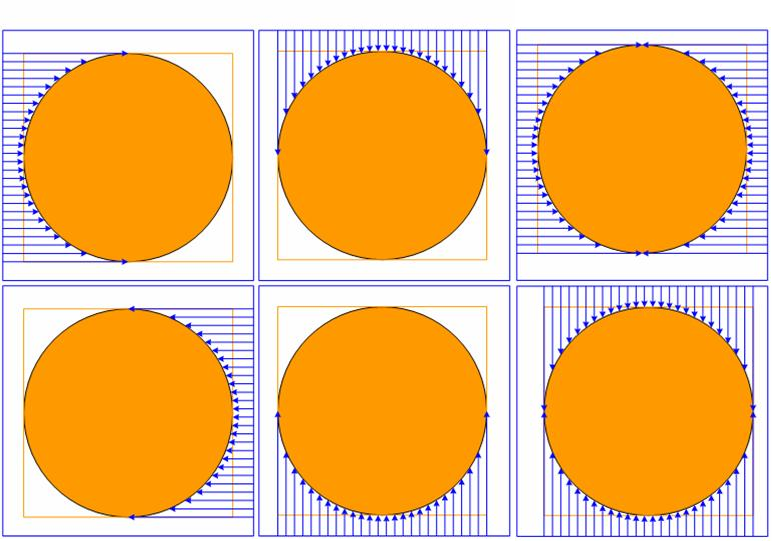
\includegraphics{stevenfigs/objectBall3.png} }
    \caption{Ball scanning directions,  (top left) left to right, (middle left) right to left, (bottom left) left and right to centre, (top right)  top to bottom, (middle right) bottom to top, (bottom right) top and bottom to centre.}
    \label{fig:objectBall3}
\end{center}
\end{figure}

Once a circle has been fit to these points, the validity of the fit circle is determined. If the diameter of the circle is significantly lower that the width of the blob then it is assumed that the circle fit is not correct.


\subsection{Goal Recognition}

With the use of soft colour classification and due to obstructions on the field, the goal is often not seen as a single blob, but rather a cluster of blobs. A scan method was used on clusters to detect the gap type and calculate the width of posts. 3 horizontal scan lines were used to detect gap type and post width by measuring the pattern of colour and soft colour compared to non object colours.

Gap types detected are: no gap (unknown post), left (right post), right (left post), middle (both posts, no crossbar), bottom (both posts and crossbar) or undefined. 

Three main variables were used to calculate goal confidence. Correct pixel to size ratio, cluster height to width ratio and goal gap detected. The amount of correct pixels required to pass as a goal object depends on the size and shape of the cluster and also what gap type it has. For instance an image of a single up close goal post will be detected as having no gap. Then it must pass a height to width ratio check and colour pixels to size ratio check to be recognised as a post. The ratio of correct pixels to size is different for each gap type.
 
\subsubsection{Goal Distance, Bearing and Elevation Calculations}

The raw distance of the goal is found by using the width of a post. With the new tall goals and the robot camera position looking down for a ball, the goal height is unreliable. If both goal posts are seen both widths are used to calculate the distance to each post. 

The raw bearing and elevation are found using the centre of the post. The method to find the centre of the post varies depending on the gap type. As with the ball these raw distances are translated back so they are relative to the hips of the robot. The elevation is not very reliable as the top of the post is often not seen.

%\subsection{Robot Recognition}
%
%Red robots are detected by clusters of red blobs. Blue robots are detected using the clusters of shadow blue blobs if blue goal tests have failed.





\subsection{Line and Corner Point Detection}

This year the algorithm used in previous years to detect field lines and corners  [Quinlan \emph{et al.}, 2006] was ported from the Aibo to the new Nao system. This required rewriting the function that transforms the found corner points in the camera plane to the field plane to suit the new robot kinematics and camera perspective. Otherwise, the algorithm is the same as the previous years for detection. Further development this year involved uniquely identifying these found corner points for use in Localization.

\subsubsection{Line Detection}
The detection of field lines is approached in a completely different manner to that of other Objects. When searching for objects, sections of a specific colour are joined together to form a blob. While this works well for most objects, white causes problems due to its abundance in the image and hence is normally ignored. Also the thin nature of lines, and the robot's low Point Of View, makes missing pixels very common within the classified image. Finally the storing of blobs, as a square which bounds the entire object, does not store enough important information about the line.

To overcome these issues the detection of lines is based around the two unique features that field lines have; their long thin length and their green-white-green transitions. Using these two details the image can be sparsely searched, since the search line does not need to find every point of the line, just enough to re-create the line. Also the transition information allows many white pixels to be thrown out early in the detection process, thereby reducing the overall load on the processor. This reliance on points and not the entire line also allows the lines to be partially hidden behind another object without effecting their detection. 

With these factors in mind, the image can now be efficiently searched in the following steps;

\begin{itemize}

\item 	The image is searched using a horizontal and vertical search grid. The search is restricted to the area in the image below the horizon line and picks out points of sharp contrast which have green-white then white-green transitions. These points are recorded in an array for later use.

\item The found points are then checked against each other to form possible lines. Once candidates are found, more points are checked and added until a line is formed. All checks on the lines at this stage is done based on gradient to allow the fastest line formation.

\item The lines are cleaned up to make sure all points actually fit on the line. Lines which have too large a number of points not contained within the final line are removed.

\item Lines are checked against each other to confirm that they are not just segments of larger lines. The allows lines to be formed that have a break in the middle, such as when a robot is on top of the line.

\item Corner points are found by extending lines and finding their intersection locations. The intersections are checked to confirm virtual points are not found. 

\item An attempt is made to uniquely identify corner points from other objects within the image. While this is not always needed, if a unique identification is made the use of the corner point within localisation becomes much more efficient.

\end{itemize}

\subsubsection{Corner Point Detection}
The locating of these corner points alone in each frame is not enough to localize with as there are numerous type-L and type-T corners on each side and a complete mirror image of the field lines on each half end of the field. Unique identification of each corner point is required in our system. A rule based approach was used to perform this identification that filters out the possible corner identity based on what properties of the corner can be extracted from the image and in most cases also some vague knowledge of robot location and orientation. 

The goal was not to provide data that Localization can rely upon solely but to fine tune the accuracy once approximate localization has been established. However this use of knowledge of location and orientation creates a loop between the Line Detection and Localization system components. This allows for the possibility of each component validating each other's incorrect data to exist. This being the case, the main focus was to write identification rules that are strict enough to eliminate the possibility of false positives. Also, the corner point identification rule written would block (that is, return an unknown corner or T point) unless the Localization confidence first came within 2 standard deviations of the probable orientation.
      
The identification relies upon the orientation of the seen corners, the combination of these corners and other lines in the image and the number of corners and lines seen. The Line Detection algorithm classifies each corner as either a type L or T and then attributes it with one of four possible orientations, pointing up/down or pointing left/right. By disassembling the field lines in the image they could be examined for what types of corners and orientations make up what is seen. Following that, this information is then decoded to match what should be seen from the present known location. Avoiding false positives here partially takes care of itself as if the robot location or orientation data is wrong, the corresponding corner orientation classification will not match the rule.

For example, in Figure \ref{fig:corner}a taken from the simulator, the detection algorithm reports seeing 3 corners: 2 type L's of orientation 2 and 4, 1 type T of orientation 1 and 4 lines. This set of data is almost unique when compared to the other countless possible positions and perspectives from which to view the field lines and can therefore be decoded with brute force. 
 
The only other occurrence is a duplicate on the opposite end of the field as both halves are identical. This the leaves the question, "which end of the field is the robot in?". Knowledge of the robots orientation could also solve this problem of determining which end of the field this scene is taken from. To be robust, the rules written require Localization to be certain of both field XY position and orientations to 2 standard deviations. This value could be increased in this case but for others closer to the mid field line, the probability of error increases as the two mirror images from each end come closer together. The necessity for this prior knowledge is best show pictorially.
    
In the first frame we have no other information to work with other than the lines themselves. In the second frame, the Goal Detection provides Localisation with enough information to determine which end of the field the robot is in and it is now possible to uniquely identify the corner points.
      
Another example of an identification rule would the identification of a mid field T corner. Conditional tests for seeing only: 2 field lines, corner count = 1, corner type = T, corner orientation = 3, robot X location is greater than zero, orientation is 135 degrees plus or minus 80 degrees and no goal post is seen, accurately reports the correct corner and filters out all others.
      
Unique identification rules were written for each corner for a selection of possible perspectives and rigorously tested in the Webots simulator. Possible sources of error discovered in testing were the extension of the penalty box line to join the side field line to create a phantom type T corner, the clipping of a type T corner into a type L by the edge of the camera frame and the center circle appears as a collection of many corners (for example an octagon). Each of these sources of error were reliably filtered out by the corner combination decoding.
      
The simulation testing also showed great improvement in Localisation over simply relying upon goal detection alone. Once a goal had been seen and Localisation determined to some approximate area, the line detection would report a unique corner point and fix a very accurate position and orientation and maintain it while looking all around the field. 

The identified point on the field is then sent to Localization after performing the following transformation.

$V_{cam}=[focLength, (IMG_{width}/2)- X_{img},(IMG_{height}/2)-{Y_{img}}]$

Transformation through neck

\textbf{$V_{1}$}=\textbf{$V_{cam}$}*\textbf{$M_{camTilt}$}

\textbf{$V_{2}$}=\textbf{$V_{1}$}*\textbf{$M_{camPan}$}

Transform body tilt

\textbf{$V_{3}$}=\textbf{$V_{2}$}*\textbf{$M_{bodyTilt}$}

$\alpha=-Chest Height/V_{3}[2]$

$distance=\alpha*\sqrt{V_{3}[0]^2+V_{3}[1]^2}$

$bearing=arctan2(V_{3}[0],V_{3}[1])$

This inter system approach to the corner identification is shown in Figure \ref{fig:corner} b and c. Green components demonstrate an improvement to this approach where one of the Localisation reset triggers becomes an external one based on an added component that monitors for robot relocation by hand by way of accelerometer readings (Teleport Detection if image is BW). In the Robocup competition robots do get picked up and moved, possibly to the other side of the field and turned around by 180 degrees when being penalized. The loop created between the Line Detection and Localisation could slow down the reset as it would take some time for the bad data to be dumped after locating a goal post and dealing with conflicting information. A specialised system component could ensure this does not happen.
\begin{figure}[htpb]
\begin{center}
    %\leavevmode
    \scalebox{0.3} {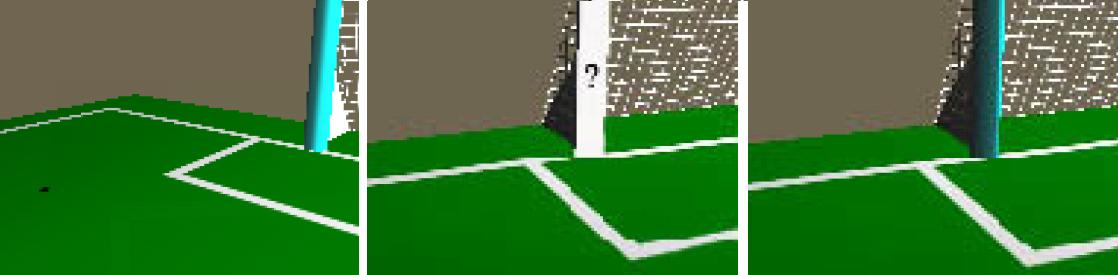
\includegraphics{alexfigs/corner.png} }
    \caption{Images of corners for examples.}
    \label{fig:corner}
\end{center}
\end{figure}

%\subsubsection{Code Implementation}
%Up until this year, Line Detection was a collection of functions within the Vision class itself. To
%reduce coupling, the Line Detection function and supporting functions were removed from the vision
%class and placed into a newly created Line Detection class. This Line Detection class is responsible for
%both line detection and the corner identification. These routines are still part of the vision system and
%the files can be found in the vision directory. No other NUManoids system component is dependent
%upon this Line Detection class to in order run and therefore it may be removed from the project build by
%editing the MakeFile in the root of the code body.
%Once a Line Detection object has been instantiated, the Line Detection function �formlines()� is
%called at the end ProcessFrame() within the class Nao. It requires no data to be passed into it and it
%outputs its results by directly modifying the elements found in the �fieldObjects� structure. The list of all
%possible corner points that can be evaluated can be found in the FieldObject.h file.
%\begin{figure}[!ht]
%\begin{center}
%    %\leavevmode
%    \scalebox{0.3} {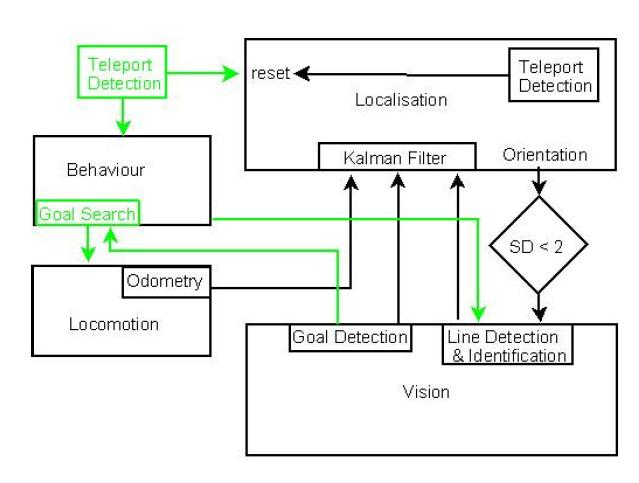
\includegraphics{alexfigs/flow.png} }
%    \caption{Software flow diagram.}
%    \label{fig:flow}
%\end{center}
%\end{figure}


\subsubsection{Penalty Spot Detection}
Penalty spots exists in two positions on the field. By detecting any penalty spot, localisation module has a higher chance of knowing where the robot is currently situated on the field. Detecting the penalty spot consists of a search heuristic:
\begin{itemize}
\item Find lines that are less then a quarter length of the screen: If a standing robot should see a penalty spot, it should be relatively small on the screen.
\item Using the points on the selected line, we scan around each of these line points for surrounding white colours:
This scan consists of a 3x3 grid search around the selected point.
\item If there does not exist to be any white colours, its most likely to be a penalty spot, Otherwise it is not a penalty spot.
\end{itemize}
This is a simple and efficient heuristic, because the priori conditions make the search space is very small.

\subsubsection{Centre Circle Detection}
Centre circle is an a very important field object on the SPL field. This object is so big that almost from any section of the field (provided that is facing inwards). It enhances and assists the localisation module greatly, due to its visibility and unambiguous properties of the object. To detect a centre circle, there exists two steps. First Step, is to remove points that do not belong on the centre circle. Second step, consists of an least squares approach to fit the points of the centre circle to an ellipse equation.
Once this is complete, we are able to obtain the ellipse, and the robots current distance to it.

The first step is removing points that do not belong on the centre circle, this is achieved by an heuristic. Here we assume that after all points have been fitted to a line, corners (intersections) of lines have been calculated and all penalty spots have already been detected. Here we assume a centre circle consists of many small straight lines, with many straight lines these should intersect on screen a large number of times. Assuming a number of corner tolerance of six, if the number of corners are greater then six, centre circle detection will be triggered. 
\begin{itemize}
\item Find the longest line (most likely to be the centre line) and remove it from the search list.
\item Find the Penalty Spot lines and remove it from the search list.
\item Assuming that the lines are small, we select all the small lines. For our system, a small line is a line that is less the image width.
\item We then select the line points that exist within these lines and store them in a vector ready to be processed by the next stage.
\end{itemize}

The next stage consists of fitting the obtained points to an ellipse equation. By fitting the points to an equation we are able to generalise and efficiently store the data of the ellipse for later use. The ellipse fitting algorithm is an implementation of 
\section{Localisation and World Modelling}
\label{sec:Localisation}
The localisation for 2009 was based on the Unscented Kalman Filter (UKF) used in 2008 !REFERENCE!. A number of extensions were 
made to improve upon the previous years implementation. These changes were made to both include new information that was available due to advances in vision, as well as to make use of ambiguous data that was not previously usable.

\subsection{Multiple Models}
The current robocup field contains many ambiguous points of reference as can be seen in \autoref{fig:LocalisationPoints}. When multiple ambiguous points are found it is possible to use a simple decision tree to determine which objects these are, however there are often times where this is not possible. The UKF was therefore extended to incorperate multiple models to allow for the use of ambiguous measurements.

The basic idea is that when an ambiguous object is seen e.g. a yellow goal post, we can determine that there are a number of possible fixed objects that could have been seen, in this example the left yellow post or the right yellow post. Using a multiple models approach the current model cloned to create as many models as there are options, in our example two. One model is then updated with the first option the next model with the second and so forth.

As these updates are done an \emph{alpha} variable is modified depending on how well the update fits the previous model. The larger the discrepancy the more the \emph{alpha} value is reduced. Therefore the model with the largest \emph{alpha} value following the update can be deemed to have been updated with the most likely option and therefore will be the most correct model. This process can be repeated for multiple ambiguous options and therefore the results of all possible combinations can be found.

If this process were repeated again and again, we would end up with an exponentially growing collection of models. Therefore it is also necessary to merge these models, combining two models into one. Merging is done so that information is not lost. Models are merged based on the following metric !REFERENCE!.

\begin{figure}[htpb]
\begin{center}
   \leavevmode
    \scalebox{0.5} {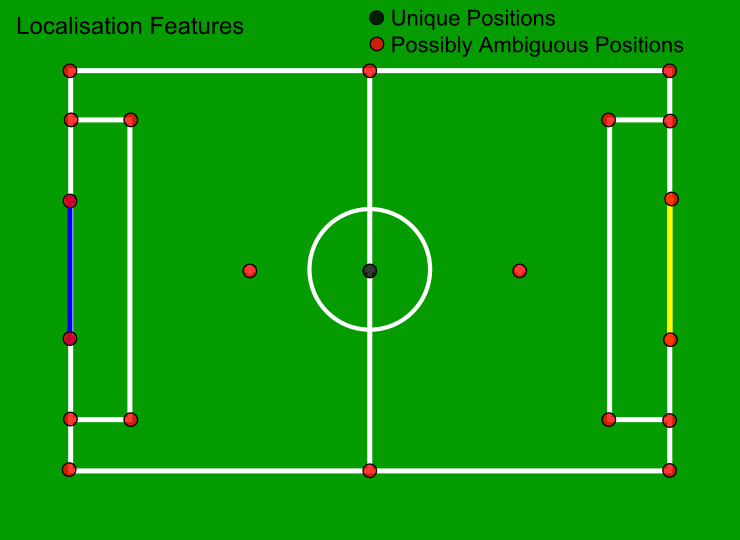
\includegraphics{figs/LocalisationPoints.png} }
    \caption{Available localisation landmarks}
    \label{fig:LocalisationPoints}
\end{center}
\end{figure}

\subsection{New Objects}
Some new objects were available as inputs for localisation this year that were not available in previous years. These included the centre circle and the penalty spots. These newly available landmarks saw huge improvements in positioning when in the mid-field area as there was previously a distinct lack of landmarks once you moved away from the goal areas. The middle of the center circle provides one of the few unique landmarks available. While the penalty spots can represent one of two locations and therefore make use of multiple models if simple hueristics prove fruitless.

\section{Behaviour}
\label{Behaviour}
\subsection{Field Player Strategy}
The overall strategy for this year was to attempt to kick the ball towards the attacking goal as quickly and as often as possible. To do this the general behaviour was to walk to the kicking position where the attacking goal was lined up and then kick. Since we only kicked forward this was a calculated position based on the position of the ball on the field. In terms of team behaviour, we attempted to always have one robot chasing the ball while any other robots tried to move into their ideal position. In an attempt to simplify the writing of behaviour code the walk engine included many planning functions so that behaviours simply pass the walk engine the desired relative position and heading and the walk engine will take it there. These path planning paths were built around the desired behaviours so many complex decisions were not required. For example when approaching the ball from the front, and therefore a large heading change is required, to prevent the robot walking through the ball on its way to the kicking position a path containing an arc walk is used to move behind the ball and correct the heading. To carry out our overall strategy a number of sub-behaviours were developed. These were run depending on the robots current circumstances as shown in ~\autoref{fig:PlayerTaskDecision}.

\begin{figure}[htpb]
\begin{center}
   \leavevmode
    \scalebox{0.8} {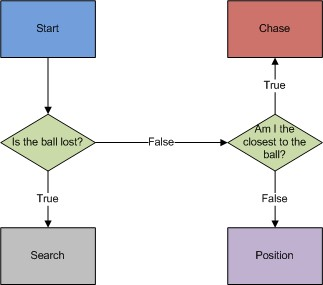
\includegraphics{figs/FieldPlayerTaskDecision.jpg} }
    \caption{Player task decision tree}
    \label{fig:PlayerTaskDecision}
\end{center}
\end{figure}



\subsubsection{Searching}
The trigger for searching was greatly improved upon from last year. Previously the robot would search if it could simply not see the ball. However when moving into position we found that it may be advantageous to lose sight of the ball for short amounts of time to gain an increase in walking speed. Because of this some high level properties were created \emph{isBallLost} and \emph{amILost}. The \emph{isBallLost} property takes into account the number of vision frames since the ball was last seen as well as the current world model uncertainty to determine if yourself or the team as a whole has lost the ball. Because the world model ball also includes information from team mates if they are providing the robot with good estimates of the ball position it may not be required to search. Likewise if the world model uncertainties indicate that the predictions are accurate searching again may not be required. The \emph{amILost} property was used to determine the validity of the robots field location estimates. Once the uncertainty reached a predefined threshold the robot would attempt to localise by doing a pan at a level likely to see the goal posts and field lines.

Once we had determined that a ball was lost and must be found we used a simple searching method. The robot would pan its head vertically from top to bottom while turning in a circle. The horizontal angle of the camera was set to one step worth of a turn towards the turning direction so that if a ball is seen at the completion of the next turn step it can begin moving forwards towards it. We would alternate cameras for each turn starting with the camera we deemed most likely to see the ball based on its estimated distance. However this sometimes proved frustrating since it would sometimes choose the wrong camera and would then require more than a complete turn to find the ball.


\subsubsection{Chasing}
The chasing behaviour is the main part of our game play. It involves walking to an ideal kicking position. turning to line up the goal, then lining up the ball and finally kicking. To simplify the writing of behaviours we created another high level property \emph{isOpponentsGoalLinedUp}. This is determined very simply, if the left hand post of the attacking goal is on our left and the right hand post is on our right then the goal is lined up for a kick. There were a number of states in the chasing behaviour. The transition conditions between states can be found in \autoref{fig:ChasingStateDiagram}.
\begin{enumerate}
\item \textbf{Approach} The robot will move towards the desired kicking position. This is situated on the opposite side of the ball to the attacking goal.
\item \textbf{Position} The robot will turn to face the attacking goal, lining it up so that it is facing between the two posts.
\item \textbf{Kick} The robot will line one of its feet up to the ball. One the ball is within the effective kicking range the kick sequence will be called.
\end{enumerate}

\begin{figure}[htpb]
\begin{center}
   \leavevmode
    \scalebox{0.8} {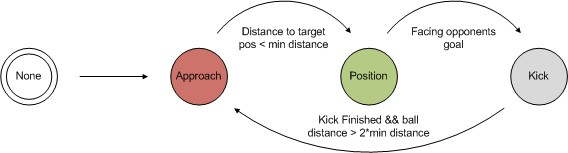
\includegraphics{figs/FieldPlayerChasingStates.jpg} }
    \caption{Chasing behaviour state diagram}
    \label{fig:ChasingStateDiagram}
\end{center}
\end{figure}

\subsubsection{Positioning}
The positioning behaviour simply moves to a fixed point on the field. Once close to the desired field position the robot turns to face the ball. If the ball can be seen the robot will track the ball. If not the robot will face towards the estimated ball position and pan to look for the ball and view localisation landmarks.

\subsection{Goal Keeper Strategy}
The overall goal keeper strategy was to keep the ball from entering the defending goal. This would ideally be achieved by using the goal keeper as an obstacle in the direct path between the ball and the defending goal. If the ball was far away, the goal keeper would spend most of its time searching (same as field player) and positioning between the ball and the defending goal. However, if the ball was close to the goalkeeper, the goal keeper would have to react by either clearing the ball (lining up for a kick towards the attacking goal) or if the ball was moving towards the goal keeper, it would perform a dive to stop the ball from entering the goal. The following subsections will describe in detail the positioning and reactions to the ball. The goal keeper has a higher priority in the over all team behaviour hierarchy. The reasoning behind this is that around the defending goal area, the ball can easily move into an area off limits to a field player, and in this situation the defending the goal is the teams main priority. A decision tree of the goal keeper can be see in ~\autoref{fig:GoalKeeperDecision}.

\begin{figure}[htpb]
\begin{center}
   \leavevmode
    \scalebox{0.8} {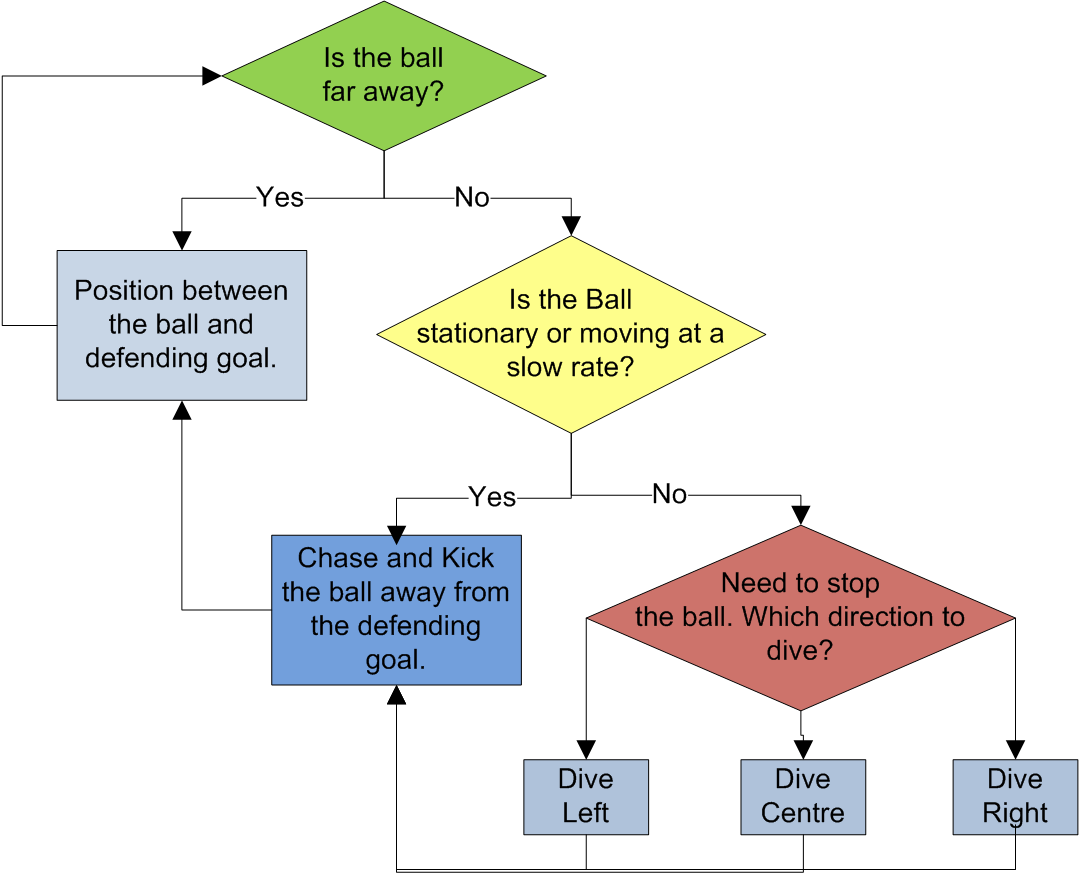
\includegraphics{aaronfigs/GoalKeeperDecisions.png} }
    \caption{Goal Keeper task decision tree}
    \label{fig:GoalKeeperDecision}
\end{center}
\end{figure}

\subsubsection{Positioning}
Unlike other teams in the competition who would simply position their goal keeper in the middle of the goals, we chose to use a more active and aggressive keeper. The positioning module was significantly different to the field player, as the goal keeper is required to attempt to position between the ball and the defending goals at all times. It heavily depended on the localisation information and current position of the ball. Using this information we calculate a position on the field to guard that maximises the coverage of the goal. This was achieved by calculating the ideal path from the ball to the centre of the goals and intersecting this ideal ball path with a boundary, where the boundary is the edge of an area for which we would like the goal keeper to roam with-in.


\subsubsection{Reactions to the Ball}
Once the ball is at a close distance, the goal keeper will react in one of two ways. 

The first is to chase and remove the ball from its defending area in the direction of the attacking goal in a similar manner as the field player. This is only triggered if the ball is stationary or moving very slowly.

The second is a dive which is triggered by a moving ball. When a dive is triggered, the goal keeper will select the best dive from three pre-written dive scripts. There are three dive scripts, Left, Forward and Right. The goal keepers dive selection criteria includes, projecting the ball to intersect its' vertical plane, then selecting the dive that closely corresponds to the intersection. The dive is executed before the ball intersects the goal keeper, so it is able to dive into position to block the balls path. The dive is within required regulation, as it only stays in its dived position for a few seconds before getting up. After the dive it will proceed to chasing and kicking the ball out of the goal area.

\section{Locomotion}

The walk used at RoboCup 2009 was a modified version of Aldebaran's walk that implemented pseudo omni-directional capabilities. Essentially, ALMotion was used to generate a set of predefined steps offline, the cached steps are then linked together online by our walk engine. This allowed the robot to walk on an arc of varying radius without stopping, and in some cases link turning steps with arc or straight steps. However, in some instances the robot still needs to stop when changing directions, for example, to change from a forward walk to a sideward walk first requires the robot to stop.

The walk engine is controlled via a \texttt{walkToPoint} interface to continuously specify a target position. A heuristic path planning algorithm was implemented to determine a fast way to get to the target point given the limited number of available steps. Paths consisting of permutations, with repetition, of the set of walk primitives (forward, arc, turn, backward and sideward) are trialled, the fastest permutation that goes through the desired target with the desired orientation is chosen. This process is repeated every time a new step is required, and the step which best implements the chosen path become the next step.

The source code for the walk engine is available as a standalone module at \href{http://github.com/soneoed/naowalkoptimiser}{http://github.com/soneoed/naowalkoptimiser}. The source release includes many things; the code to generate and cache the steps, the code for the walk engine itself, the scripted motion files for kicks, getups and saves, the fall-preservation control, and code used to optimise the joint stiffnesses as a function of gait cycle (along with the associated laser scanner robot tracking).

\subsection{Pattern Generation}

Aldebaran's ALMotion was used to generate walk primitives in the following directions; forward, arc, turn, backward and sideward. The arc primitive contains steps on arcs of radii from 5cm to 100cm in 5cm increments, and the turn primitive contains steps on turns of angle from 9 degrees to 180 degrees in 9 degree increments. The forward, backward and sideward only contain a single set of steps, in particular, only steps of a single length are possible while walking forwards or backwards, making lining up kicks difficult.

A walk primitive contains a set of steps. A set of steps includes steps for both left and right legs, and a start step, a second step, a normal step, and a stop step. If the walk primitive contains many directions, that is, an arc or turn walk primitive, there is a set of steps for each direction. Consequently, there are over 800 individual cached steps used by the walk engine, and they are organised as shown in \autoref{fig:LocomotionSteps}.

\begin{figure}[tbh]
	\begin{center}
		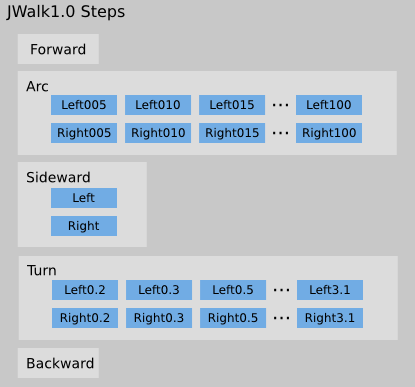
\includegraphics[width=0.6\textwidth]{locomotionfigs/steps.png}
		\caption{The organisation of cached steps used by the walk engine.}
		\label{fig:LocomotionSteps}
	\end{center}
\end{figure}

Each walk primitive has its own set of slightly different walk parameters, and in the case of arcs, a slightly different set of parameters was given based on the arc radius. The walk parameters are shown in \autoref{fig:LocomotionWalkParameters}.

\begin{figure}
	\begin{center}
		{\scriptsize\begin{verbatim}
		configureForwardWalk()
		   setWalkParameters(0.060, 0.012, 0.04, 0.5, 0.013, 0.007);
		   setWalkExtraParameters(4, -4, 0.23, 1.5);
		   setWalkGaitPeriod(23);
		   setWalkArmParameters(90*TO_RAD, 15*TO_RAD, 20*TO_RAD, 10*TO_RAD);

		configureBackwardWalk()
		   setWalkParameters(0.030, 0.012, 0.04, 0.5, 0.015, 0.012);
		   setWalkExtraParameters(4, -4, 0.23, 1.5);
		   setWalkGaitPeriod(24);
		   setWalkArmParameters(90*TO_RAD, 15*TO_RAD, 20*TO_RAD, 10*TO_RAD);

		configureArcWalk()
		   if (radius < 8)
		      setWalkParameters(0.030, 0.012, 0.04, 0.5, 0.013, 0.007);
		      setWalkGaitPeriod(22);
		   else if (radius < 12)
		      setWalkParameters(0.035, 0.012, 0.04, 0.5, 0.013, 0.007);
		      setWalkGaitPeriod(22);
		   else if (radius < 17)
		      setWalkParameters(0.040, 0.012, 0.04, 0.5, 0.013, 0.007);
		      setWalkGaitPeriod(22);
		   else if (radius < 42)
		      setWalkParameters(0.045, 0.012, 0.04, 0.5, 0.013, 0.007);
		      setWalkGaitPeriod(22);
		   else
		      setWalkParameters(0.065, 0.012, 0.04, 0.5, 0.013, 0.007);
		      setWalkGaitPeriod(24);
		   setWalkExtraParameters(4, -4, 0.23, 1.5);
		   setWalkArmParameters(90*TO_RAD, 15*TO_RAD, 20*TO_RAD, 10*TO_RAD);

		configureTurn()
		   setWalkParameters(0.060, 0.012, 0.04, 0.3, 0.01, 0.011);
		   setWalkExtraParameters(4, -4, 0.23, 1.5);
		   setWalkGaitPeriod(21);
		   setWalkArmParameters(90*TO_RAD, 15*TO_RAD, 20*TO_RAD, 10*TO_RAD);

		configureSideWalk()
		   setWalkParameters(0.060, 0.012, 0.04, 0.5, 0.00, 0.011);
		   setWalkExtraParameters(4, -4, 0.23, 1.5);
		   setWalkGaitPeriod(20);
		   setWalkArmParameters(90*TO_RAD, 15*TO_RAD, 20*TO_RAD, 10*TO_RAD);
		\end{verbatim}}
		\caption{The walk parameter's for Aldebaran's ALMotion walk used to generate the cached steps.}
		\label{fig:LocomotionWalkParameters}
	\end{center}
\end{figure}

As with last year's walk engine \cite{JasonsAcraPaper} different joint stiffnesses were given to each joint, the stiffnesses were slightly updated for the new V3 NAO. The stiffnesses for every joint, except the two head joints, for each primitive are shown in \autoref{fig:LocomotionWalkParameters2}.

\begin{figure}
	\begin{center}
		{\scriptsize\begin{verbatim}
		forward =  [0.10, 0.25, 0.10, 0.25, 0.70, 0.26, 0.55, 0.25, 0.24, 0.28]
		backward = [0.10, 0.25, 0.10, 0.25, 0.70, 0.26, 0.55, 0.25, 0.23, 0.25]
		arc =      [0.10, 0.25, 0.10, 0.25, 0.70, 0.26, 0.55, 0.25, 0.23, 0.25]
		sideward = [0.10, 0.25, 0.10, 0.25, 0.70, 0.35, 0.55, 0.25, 0.23, 0.25]
		turn =     [0.10, 0.25, 0.10, 0.25, 0.70, 0.26, 0.55, 0.25, 0.23, 0.25]
		\end{verbatim}}
		\caption{The joint stiffnesses for each joint for each walk primitive used by the walk engine. The left arm and left leg stiffnesses are shown, but the same values are used for the right side.}
		\label{fig:LocomotionWalkParameters2}
	\end{center}
\end{figure}

\subsection{Step Linking}

The linking of steps to form a walk is simplified by having each walk primitive store each set of steps in a linked list. Basically the linked list is set up so that each step knows which step would follow if no direction change is required, and which step is required to bring the robot to rest. The linked list representation of a walk primitive is shown in Figure \ref{LocomotionLinkedSteps}.

\begin{figure}[tbh]
	\begin{center}
		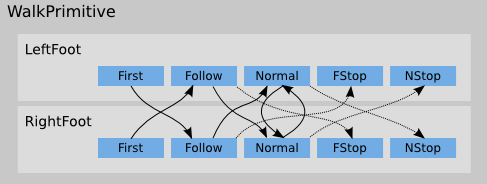
\includegraphics[width=0.6\textwidth]{locomotionfigs/linkedsteps.png}
		\caption{The organisation of a walk primitive used by the walk engine.}
		\label{LocomotionLinkedSteps}
	\end{center}
\end{figure}

A change in direction is essentially a transition from one walk primitive's linked list to the new direction's linked list, being careful to enter the new list at the correct point. There are several complications, the first is direction changes that first required the robot to stop. This is accomplished simply by selecting the appropriate stopping step, subsequent calls to walkToPoint will automatically select the first step in the new direction. The second complication is that many steps come in pairs, for example, walking on a rightward arc has a right and then a left step that must follow; calls for direction changes are ignored until the left step is completed. 

\subsection{Path Planning}

In order to maximise the utility of the walk engine given the limited number of available primitives a simple time-based heuristic path planning algorithm was implemented. Prior to the selection of every step the time taken by between 4 and 6 different candidate paths to reach the target position and orientation is calculated. The path with the shortest time is selected, and the next step is chosen to implement that path as closely as possible given the current pose of the robot.

The candidate paths consist of straight, arc, sideward, and turn segments.  In particular, for path planning with a final orientation, the candidate paths are arc-straight-arc, turn-straight-turn, turn-backward-turn and turn-sideward-turn, where the initial and final turn and arc segments may not be required. \autoref{fig:LocomotionPathPlanning} shows examples of the planned paths. Additionally, paths could be planned ignoring the final orientation.

\begin{figure}[tbh]
	\begin{center}
		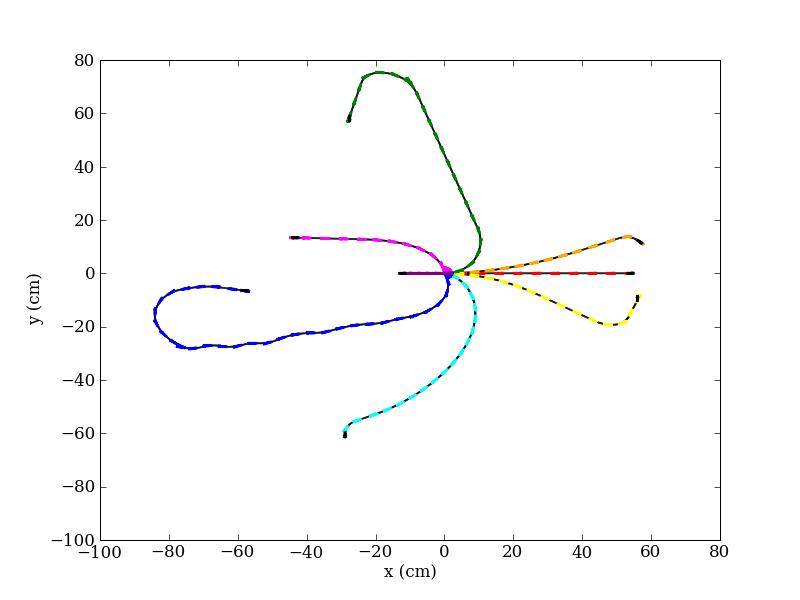
\includegraphics[width=0.8\textwidth]{locomotionfigs/pathplanning.png}
		\caption{A selection of planned paths for different target locations and orientations. The target location and orientation is shown for each path with a black arrow. The orientation and position of the simulated robot is shown with the coloured arrows for each path. Note that if the target locations were balls, the calculated paths avoid the ball.}
		\label{fig:LocomotionPathPlanning}
	\end{center}
\end{figure}

\subsection{Scripted Motion}
\subsubsection{Getups}
We have two getups; one for when it is lying on its chest, and another for when it is on its back. We found that Aldebaran's getup from front included with Choregraphe broke the HipYawPitch motor frequently. Consequently, we created a new one from scratch so that it was easier on this fragile joint. The motion also turned out to be slightly faster, but just as reliable. 

The getup from back was simply Aldebaran's script from Choregraphe.

\subsubsection{Kicks and Saves}
We have five kick scripts for each foot; two forwards, two sidewards and one backwards. The duplicate kicks target balls at different relative positions, for example, the two forward kicks are designed to kick balls close to the centre, and far from the centre. This was done to avoid need to line up kicks perfectly, especially given the limited walk engine.

We have three save scripts; a left save, a centre save and a right save. Each of the saves involves spreading the legs, for the left and right save the other foot remains on the ground making getting back up very easy. For the centre save both the left and right legs are spread, while the robot leans back on its arms,.

All of the script files for kicks and saves were generated using Aldebaran's Choregraphe. The motion script files, as a comma-separated file, are available at \href{http://github.com/soneoed/naowalkoptimiser}{http://github.com/soneoed/naowalkoptimiser}.

\subsubsection{Fall Protection Poses}
When the robot is falling over it goes into a fall protection pose to minimise damage to the robot. There are four protection poses; one for each falling direction. The forward pose attempt to have the robot land chest-first on the floor avoid damage to the arms and head, while the backward fall pose aims to have the robot land on its bottom in a sitting position again protecting the arms and head. The left and right fall poses tuck the left or right arm, respectively, into the narrow part of the torso. 

\input{communication.tex}

\section{Acknowledgements}
 \noindent The NUbots are grateful to all colleagues, friends, previous members, fans and supporters of the team including  the Faculty of Engineering and Built Environment, the School of Electrical Engineering and Computer Science, and the ARC Centre of Excellence for Complex Dynamic Systems and Control (CDSC) at the University of Newcastle, Australia.

\noindent Links to the NUbots' publications can be found at the NUbots' webpage
\begin{center}
\url{http://robots.newcastle.edu.au/}
\end{center}



\bibliographystyle{named}
\bibliography{aibo}
\end{document}
